%
%                       Documento principal main.tex
%                           Plantilla de Libro            
%                             version:  0.1.0
%      
%                               Contacto:
%                 Github:   https://github.com/medicendav
%                 Correo:   davidtorrezreyes@gmail.com   
%
%-------------------------------------------------------------------------
%
%   Copyright 2020 David Torrez Reyes
%   This file is part of BookTemplate.
%
%   BookTemplate is free software: you can redistribute it and/or modify
%   it under the terms of the GNU General Public License as published by
%   the Free Software Foundation, either version 3 of the License, or
%   (at your option) any later version.
%
%   BookTemplate is distributed in the hope that it will be useful,
%   but WITHOUT ANY WARRANTY; without even the implied warranty of
%   MERCHANTABILITY or FITNESS FOR A PARTICULAR PURPOSE.  See the
%   GNU General Public License for more details.
%
%   You should have received a copy of the GNU General Public License
%   along with BookTemplete.  If not, see <https://www.gnu.org/licenses/>.
%
%-------------------------------------------------------------------------
%
%   Organización de la plantilla:
%   
%   main.tex:
%   Carpeta:
%           Estilos:
%                   preámbulo.tex:
%                   constantes.tex
%                   entornos.tex
%                   encabezados.tex
%           Estructura:
%                   portada.tex
%                   agradecimentos.tex
%                   prefacio.tex                   
%           Capítulos:
%                   capitulo1.tex
%           Imágenes:
%                   ...
%                   Fuentes:
%           Bibliografía:
%
%--------------------------------------------------------------------------

% Definimos la clase de documento: En este caso book, con los parámetros opcionales
% definimos el tamaÑo de letra (10pt), el tamaÑo de papel (letterpaper) y el formato
% de impresión a dos lados.
\documentclass[10pt,letterpaper,twoside]{book}

% Incluimos el archivo preámbulo.tex que se encuentra en el directorio Estilos. De
% modo que cargamos todos los paquetes necesarios para la elaboración del documento.
%
%                       Preámbulo del documento
%
%           Contiene todos los paquetes necesarios para la
%                       compilación del documento
%
%-------------------------------------------------------------------------
%
%Copyright 2020 David Torrez Reyes
%This file is part of BookTemplate.
%
%BookTemplate is free software: you can redistribute it and/or modify
%it under the terms of the GNU General Public License as published by
%the Free Software Foundation, either version 3 of the License, or
%(at your option) any later version.
%
%BookTemplate is distributed in the hope that it will be useful,
%but WITHOUT ANY WARRANTY; without even the implied warranty of
%MERCHANTABILITY or FITNESS FOR A PARTICULAR PURPOSE.  See the
%GNU General Public License for more details.
%
%You should have received a copy of the GNU General Public License
%along with BookTemplete.  If not, see <https://www.gnu.org/licenses/>.
%-------------------------------------------------------------------------




%                  Paquetes de idiomas y codificación
%-------------------------------------------------------------------------
% El paquete inputenc modifica la codificación de entrada de LaTeX.
% Permite escribir con acentos, símbolos inusuales, etc. Como parámetro 
% opcional ingresamos la codificación deseada (latin1) ISO 8859-1.  
\usepackage[utf8]{inputenc}


% El paquete babel gestiona el idioma en el cual se desea trabajar, en
% este caso español (spanish)
\usepackage[spanish]{babel}


% El paquete fontenc gestiona la codificación de salida del documento.
% EL parámetro (T1) indica la codificación estándar de LaTeX
\usepackage[T1]{fontenc}




%                  Paquetes de gráficos, tablas
%-------------------------------------------------------------------------
% El entorno multicol, es de gran utilidad en los sitios donde se
% quieren poner dos figuras una al lado de la otra.
\usepackage{multicol}


% El entorno tabularx, sirve para hacer tablas con  párrafos sin tener que
% indicar  el ancho  de cada  columna de párrafo particular.
\usepackage{tabularx}

% Paquete necesario para la adición de figuras.
% Con el comando \graphcspath indicamos el directorio en el cual se encuentran
% las imágenes a utilizar 
\usepackage{graphicx}
\graphicspath{{Imagenes/}}




%                 Paquetes de configuración de paginas 
%-------------------------------------------------------------------------
% Paquete geometry, gestiona los margenes del documento.
\usepackage[top=3cm,bottom=3cm,left=3cm,right=3cm]{geometry}
\usepackage{lipsum}



%                 Paquetes para la gestión de colores 
%-------------------------------------------------------------------------
% EL paquete xcolor, necesario para la creación y uso de colores.
\usepackage{xcolor}




%     Paquetes para la creación de ecuaciones y simbología matemática 
%-------------------------------------------------------------------------
% Paquetes necesarios para introducir simbología matemática, ecuaciones,
% teoremas, etc.
\usepackage{amsmath}
\usepackage{amsfonts}
\usepackage{amssymb}
\usepackage{amsthm}


% Incluimos el archivo entornos, donde definimos entornos o ambientes creados
% por mi, como frases Celebres, observaciones, etc.
%
%                           	Entornos
%
%           Contiene los comandos necesarios crear nuevos ambientes
%        o entornos de trabajo como frases celebres, observaciones, etc
%
%-------------------------------------------------------------------------
%
%Copyright 2020 David Torrez Reyes
%This file is part of BookTemplate.
%
%BookTemplate is free software: you can redistribute it and/or modify
%it under the terms of the GNU General Public License as published by
%the Free Software Foundation, either version 3 of the License, or
%(at your option) any later version.
%
%BookTemplate is distributed in the hope that it will be useful,
%but WITHOUT ANY WARRANTY; without even the implied warranty of
%MERCHANTABILITY or FITNESS FOR A PARTICULAR PURPOSE.  See the
%GNU General Public License for more details.
%
%You should have received a copy of the GNU General Public License
%along with BookTemplete.  If not, see <https://www.gnu.org/licenses/>.
%-------------------------------------------------------------------------


%                       Mis Entornos
%----------------------------------------------------------------------------
% La sintaxis para la definición de entornos nuevos es
%
% \newenvironment{ENTORNO}[ARGUMENTOS]{ANTES}{DESPUÉS}
%
% En ANTES escribiremos el grupo de comandos que hay que ejecutar al iniciar 
% el entorno y, por tanto, los que le darán el formato al mismo, y DESPUÉS, 
% los que se activarán tras el texto. El resto de elementos funciona como antes.
%-----------------------------------------------------------------------------




%                       Frases Celebres
%%%%%%%%%%%%%%%%%%%%%%%%%%%%%%%%%%%%%%%%%%%%%%%%%%%%%%%%%%%%%%%%%%%%%%
%
% Ejemplo de uso:
% 
% \begin{FraseCelebre}
%   \begin{Frase}
%     ...
%   \end{Frase}
%   \begin{Fuente}
%     ...
%   \end{Fuente}
% \end{FraseCelebre}
%''''''''''''''''''''''''''''''''''''''''''''''''''''''''''''''''''''''
%
% Definición del entorno de Frase Celebre
\newenvironment{FraseCelebre}%
  % Entorno para crear una lista personalizada:
  % \begin{list}{Etiqueta}{Declaraciones}
  % Etiqueta: Marca de los items
  % Declaraciones: Definiciones de longitud  
  {\begin{list}{}{%
    % Definimos margen izquierdo de logitud 0.5 el espacio del texto
    \setlength{\leftmargin}{0.5\textwidth}%
    % No hay espacio extra entre párrafos de la lista 
    \setlength{\parsep}{0cm}%
    % Espacio vertical añadido al inicio y final de la lista
    \addtolength{\topsep}{0.5cm}%
    }
  }
  {\unskip \end{list}}
 

% Definición del entorno de Frase
\newenvironment{Frase}%
  % Alineación a la derecha con estilo cursiva y tamaño \small
  {\item \begin{flushright}%
    \small\em}% 
  {\end{flushright}}


% Definición del entorno de Frase
\newenvironment{FraseA}%
  % Alineación a la derecha con estilo cursiva y tamaño \small
  {\item \begin{center}%
    \small\em}% 
  {\end{center}}

% Definición del entorno de Frase 
\newenvironment{Fuente}%
   % Alineación a la derecha y tamaño de letra \small   
{\item \begin{flushright}\small}%
  {\end{flushright}}
%%%%%%%%%%%%%%%%%%%%%%%%%%%%%%%%%%%%%%%%%%%%%%%%%%%%%%%%%%%%%%%%%%%%





%                       Frases Celebres Centradas
%%%%%%%%%%%%%%%%%%%%%%%%%%%%%%%%%%%%%%%%%%%%%%%%%%%%%%%%%%%%%%%%%%%%%%
%
% Ejemplo de uso:
% 
% \begin{FraseCelebreCentrada}
%   \begin{FraseCentrada}
%     ...
%   \end{FraseCentrada}
%   \begin{FuenteCentrada}
%     ...
%   \end{FuenteCentrada}
% \end{FraseCelebreCentrada}
%''''''''''''''''''''''''''''''''''''''''''''''''''''''''''''''''''''''
%

\newenvironment{FraseCelebreCentrada}%
  % Declaraciones: Definiciones de longitud  
  {\begin{list}{}{%
    % Definimos margen izquierdo de logitud 0 el espacio del texto
    \setlength{\leftmargin}{0cm}%
    % No hay espacio extra entre párrafos de la lista 
    \setlength{\parsep}{0.5cm}%
    % Espacio vertical añadido al inicio y final de la lista
    \addtolength{\topsep}{0.5cm}%
    }
  }
  {\unskip \end{list}}
% Definición del entorno de Frase
\newenvironment{FraseCentrada}%
  % Alineación centrada con estilo cursiva y tamaño \small
  {\item \begin{center}%
    \small\em}% 
  {\end{center}}

% Definición del entorno de Frase Centrada
\newenvironment{FuenteCentrada}%
   % Alineación centrada y tamaño de letra \small   
{\item \begin{center}\small}%
  {\end{center}}
%%%%%%%%%%%%%%%%%%%%%%%%%%%%%%%%%%%%%%%%%%%%%%%%%%%%%%%%%%%%%%%%%%%%


% Incluimos el archivo encargado de generar los encabezados
%
%                   Cabeceras y pies de pagina
%       Formato de las cabeceras de las paginas, por ejemplo
%       nombre del capitulo, sección, numero de pagina, etc.
%
%-------------------------------------------------------------------------
%
%Copyright 2020 David Torrez Reyes
%This file is part of BookTemplate.
%
%BookTemplate is free software: you can redistribute it and/or modify
%it under the terms of the GNU General Public License as published by
%the Free Software Foundation, either version 3 of the License, or
%(at your option) any later version.
%
%BookTemplate is distributed in the hope that it will be useful,
%but WITHOUT ANY WARRANTY; without even the implied warranty of
%MERCHANTABILITY or FITNESS FOR A PARTICULAR PURPOSE.  See the
%GNU General Public License for more details.
%
%You should have received a copy of the GNU General Public License
%along with BookTemplete.  If not, see <https://www.gnu.org/licenses/>.
%-------------------------------------------------------------------------


% Paquete que adminstra los cabeceras
\usepackage{fancyhdr}
% Definimos el estilo general de las cabeceras (fancy)
\pagestyle{fancy}
% Quitamos el estilo de encabezado por defecto
\fancyhf{}
% Predefinímos el comando \chaptermark para que solo nos aparezca
% el numero de Capítulo y su nombre
\renewcommand{\chaptermark}[1]{%
\markboth{\textsc{ \thechapter.}\ #1}{}}
% Predefinímos el comando \sectionmark para que solo nos aparezca
% el numero de Sección y su nombre
\renewcommand{\sectionmark}[1]{%
\markright{\thesection{} #1}{}}

%Paginas pares
\fancyhead[RO]{\rightmark}
\fancyhead[LO]{\thepage}

%Paginas impares 
\fancyhead[LE]{ \leftmark}
\fancyhead[RE]{\thepage}



\newcommand{\cabecera}[1]{%
    \fancyhead[RO]{\textsc{#1}}%
    \fancyhead[LE]{\textsc{#1}}%
}

\newcommand{\restauraCabecera}{%
    % Definimos el estilo general de las cabeceras (fancy)
\pagestyle{fancy}
% Quitamos el estilo de encabezado por defecto
\fancyhf{}

%Paginas pares
\fancyhead[RO]{\rightmark}
\fancyhead[LO]{\thepage}

%Paginas impares 
\fancyhead[LE]{ \leftmark}
\fancyhead[RE]{\thepage}
}

\newcommand{\Agradecimentos}{Agradecimientos\markright{Agradecimentos}}


% Estilo de pagina plana
\fancypagestyle{plain}{%
    \fancyhf{}
    \fancyfoot[C]{\thepage}
    \renewcommand{\headrulewidth}{0pt}
    \renewcommand{\footrulewidth}{0pt}
}


\makeatletter
\def\cleardoublepage{\clearpage\if@twoside \ifodd\c@page\else
  \hbox{}
  \thispagestyle{empty}
  \newpage
  \if@twocolumn\hbox{}\newpage\fi\fi\fi}
\makeatother

% Incluimos el archivo constantes.tex, en el cual tenemos definidos nuevos comandos
% que ayudan a simplificar la escritura del código
%
%                           Constantes
%
%           Contiene constantes definidas como nuevos comandos
%                para la rápida escritura del documento
%
%-------------------------------------------------------------------------
%
%Copyright 2020 David Torrez Reyes
%This file is part of BookTemplate.
%
%BookTemplate is free software: you can redistribute it and/or modify
%it under the terms of the GNU General Public License as published by
%the Free Software Foundation, either version 3 of the License, or
%(at your option) any later version.
%
%BookTemplate is distributed in the hope that it will be useful,
%but WITHOUT ANY WARRANTY; without even the implied warranty of
%MERCHANTABILITY or FITNESS FOR A PARTICULAR PURPOSE.  See the
%GNU General Public License for more details.
%
%You should have received a copy of the GNU General Public License
%along with BookTemplete.  If not, see <https://www.gnu.org/licenses/>.
%-------------------------------------------------------------------------


%   Titulo
%----------------------------:
% \titulo ---> \textbf{Notas de teoría cuántica de campos}
\newcommand{\titulo}{Breve introducción de la teoría cuántica de campos}


%   Autor
%----------------------------:
% \titulo ---> \textbf{Notas de teoría cuántica de campos}
\newcommand{\autor}{David Torrez Reyes}

%----------------------------------------------------------------------------
%                              Inicio del documento
%----------------------------------------------------------------------------

% Inicio del documento
\begin{document}
%
%                           	Portada
%
%           Contiene los comandos necesarios para generar la portada
%                			  del documento
%
%-------------------------------------------------------------------------
%
%Copyright 2020 David Torrez Reyes
%This file is part of BookTemplate.
%
%BookTemplate is free software: you can redistribute it and/or modify
%it under the terms of the GNU General Public License as published by
%the Free Software Foundation, either version 3 of the License, or
%(at your option) any later version.
%
%BookTemplate is distributed in the hope that it will be useful,
%but WITHOUT ANY WARRANTY; without even the implied warranty of
%MERCHANTABILITY or FITNESS FOR A PARTICULAR PURPOSE.  See the
%GNU General Public License for more details.
%
%You should have received a copy of the GNU General Public License
%along with BookTemplete.  If not, see <https://www.gnu.org/licenses/>.
%-------------------------------------------------------------------------


%----------------------------------------------
%				Primera portada
%----------------------------------------------

% Estilo de pagina vacío, No genera encabezado
\thispagestyle{empty}

% Creamos el entorno para generar portada
\begin{titlepage}
	\centering
	% Genera una linea de la longitud del texto con grosor de 1.5 pts
	\rule{\textwidth}{1.5pt} 
		% Cambio tamaño de letra grande (\huge) y texto en negritas
		% Llamamos a la constante \titulo
		{\huge\bfseries		\titulo 	\par}
	% Genera una linea de la longitud del texto con grosor de 1.5 pts
	\rule{\textwidth}{1.5pt} \par
	% Dejamos un espacio de 3cm
	\vspace{3cm}
		% Llamamos a la constante \autor y cambiamos el tamaño de letra a (Large)
		{\huge	\autor \par}
	% Deja un espacio de 3cm
	\vspace{3cm}	
		%Incluimos una imagen de portada
		{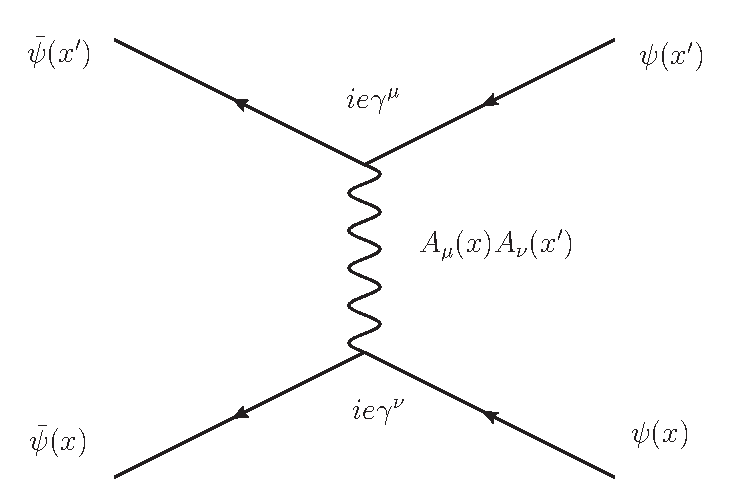
\includegraphics{diagrama_portada} \par}
		% Dejamos un espacio de 2.5cm
	\vspace{2.5cm}
		% Generamos la fecha
		{\huge	\today \par}
		% Genera una linea de la longitud del texto con grosor de 1.5 pts
	\rule{\textwidth}{1.5pt}
\end{titlepage}

%----------------------------------------------
%				Segunda portada
%----------------------------------------------

% Estilo de pagina vacío, No genera encabezado
\thispagestyle{empty}
% Creamos el entorno para generar portada
\begin{titlepage}
	\centering
	\vspace{10cm}
	% Genera una linea de la longitud del texto con grosor de 1.5 pts
	\rule{\textwidth}{1.5pt} 
		% Cambio tamaño de letra grande (\huge) y texto en negritas
		% Llamamos a la constante \titulo
		{\huge\bfseries		\titulo 	\par}
	% Genera una linea de la longitud del texto con grosor de 1.5 pts
	\rule{\textwidth}{1.5pt}
	% Termina el párrafo del titulo
	\par
	% Deja un espacio de 5cm
	\vspace{5cm}	
		{\huge Notas de Teoría Cuántica de Campos \par}
	% Deja un espacio de 5cm
	\vspace{4cm}
	% Llamamos a la constante \autor y cambiamos el tamaño de letra a (Large)
		{\huge	\autor \par}
	% Dejamos un espacio de 3cm
	\vspace{4cm}
		% Generamos la fecha
		{\Large	\today \par}
	\vspace{3cm}
		% Copyright
		{\Large \copyright{} Copyright  2020  \autor}

	\end{titlepage}


%
%                            Agradecimientos
%
%-------------------------------------------------------------------------
%
%Copyright 2020 David Torrez Reyes
%This file is part of BookTemplate.
%
%BookTemplate is free software: you can redistribute it and/or modify
%it under the terms of the GNU General Public License as published by
%the Free Software Foundation, either version 3 of the License, or
%(at your option) any later version.
%
%BookTemplate is distributed in the hope that it will be useful,
%but WITHOUT ANY WARRANTY; without even the implied warranty of
%MERCHANTABILITY or FITNESS FOR A PARTICULAR PURPOSE.  See the
%GNU General Public License for more details.
%
%You should have received a copy of the GNU General Public License
%along with BookTemplete.  If not, see <https://www.gnu.org/licenses/>.
%-------------------------------------------------------------------------




% Estilo de pagina vacío, No genera encabezado
\thispagestyle{plain}

% Dejando un espacio entre el margen superior y la frase
\vspace*{0.4\textwidth}

% Frase Celebre Centrada.... Ver entornos.tex
\begin{FraseCelebreCentrada}
  \begin{FraseCentrada}
    Nos encontramos en los comienzos mismos de la era de la raza humana.\\
    No es ilógico que tengamos o que tropecemos con problemas, \\
    pero hay decenas de miles de años en el futuro. \\
    Es responsabilidad nuestra hacer lo que podamos, \\
    aprender lo que podamos, mejorar las soluciones y \\
    transmitirlas a nuestros sucesores. \\
    Es responsabilidad nuestra dejar las manos libres a las generaciones futuras
  \end{FraseCentrada}
  \begin{FuenteCentrada}
    Richard P. Feynman
  \end{FuenteCentrada}
\end{FraseCelebreCentrada}

% Nueva pagina
\newpage



\thispagestyle{plain}
\phantomsection
\addcontentsline{toc}{chapter}{Agradecimientos}

\chapter*{Agradecimentos}
\cabecera{Agradecimentos}
\begin{FraseCelebre}
  \begin{Frase}
    Había una vez...
  \end{Frase}
  \begin{Fuente}
    MeDicenDav
  \end{Fuente}
\end{FraseCelebre}


...


\cleardoublepage
\restauraCabecera
%
%                       Preámbulo del documento
%
%           Contiene todos los paquetes necesarios para la
%                       compilación del documento
%
%-------------------------------------------------------------------------
%
%Copyright 2020 David Torrez Reyes
%This file is part of BookTemplate.
%
%BookTemplate is free software: you can redistribute it and/or modify
%it under the terms of the GNU General Public License as published by
%the Free Software Foundation, either version 3 of the License, or
%(at your option) any later version.
%
%BookTemplate is distributed in the hope that it will be useful,
%but WITHOUT ANY WARRANTY; without even the implied warranty of
%MERCHANTABILITY or FITNESS FOR A PARTICULAR PURPOSE.  See the
%GNU General Public License for more details.
%
%You should have received a copy of the GNU General Public License
%along with BookTemplete.  If not, see <https://www.gnu.org/licenses/>.
%-------------------------------------------------------------------------


\chapter*{Prefacio}
\cabecera{Prefacio}

\begin{FraseCelebre}
    \begin{Frase}
        En ciencia uno intenta decir a la gente,\\
        en una manera en que todos lo puedan entender,\\
        algo que nunca nadie supo antes.\\
        La poesía es exactamente lo contrario.
    \end{Frase}
    \begin{Fuente}
        Paul Adrien Maurice Dirac
    \end{Fuente}
\end{FraseCelebre}


...






\cleardoublepage
\restauraCabecera
    
\tableofcontents
\end{document}